%% =====================================================================
%% BÁO CÁO BÀI TẬP LỚN MÔN DEEP LEARNING
%% Tác giả : Đỗ Văn Cung – Lớp 12423TN
%% Đề tài  : Ứng Dụng Mô Hình Ngôn Ngữ Lớn Trong Phân Loại Cảnh Báo
%%            Lỗ Hổng Bảo Mật Kết Hợp Đồ Thị Thuộc Tính Mã Nguồn và
%%            Rào Chắn Chính Sách Bảo Thủ
%% Compile : lualatex hoặc xelatex  (yêu cầu font Times New Roman)
%% =====================================================================

\documentclass[12pt, a4paper]{article}

%% --- Encoding & Font ---------------------------------------------------
\usepackage{fontspec}
\setmainfont{Times New Roman}
\usepackage{polyglossia}
\setmainlanguage{vietnamese}
\setotherlanguage{english}

%% --- Page Layout -------------------------------------------------------
\usepackage[
  top=2.5cm, bottom=2.5cm,
  left=3.0cm, right=2.0cm,
  headheight=15pt
]{geometry}

%% --- Typography & Spacing ----------------------------------------------
\usepackage{microtype}
\usepackage{setspace}
\setstretch{1.5}
\setlength{\parindent}{1.25cm}
\setlength{\parskip}{0pt}

%% --- Math --------------------------------------------------------------
\usepackage{amsmath, amssymb, amsfonts}

%% --- Tables ------------------------------------------------------------
\usepackage{booktabs}
\usepackage{multirow}
\usepackage{array}
\usepackage{tabularx}
\usepackage{makecell}
\usepackage{longtable}
\renewcommand{\arraystretch}{1.3}

%% --- Graphics & Colors -------------------------------------------------
\usepackage{graphicx}
\usepackage[dvipsnames, table]{xcolor}
\definecolor{deepblue}{RGB}{0,53,107}
\definecolor{lightgray}{RGB}{242,242,242}
\definecolor{accentred}{RGB}{192,0,0}
\definecolor{accentgreen}{RGB}{0,112,44}
\definecolor{codebg}{RGB}{248,248,248}

%% --- Code Listings -----------------------------------------------------
\usepackage{listings}
\lstset{
  basicstyle   = \ttfamily\small,
  breaklines   = true,
  frame        = single,
  backgroundcolor = \color{codebg},
  rulecolor    = \color{gray!40},
  xleftmargin  = 1em,
  xrightmargin = 1em,
  aboveskip    = 6pt,
  belowskip    = 6pt,
}

%% --- Diagrams (TikZ) ---------------------------------------------------
\usepackage{tikz}
\usetikzlibrary{shapes.geometric, arrows.meta, positioning, fit, backgrounds, calc}
\tikzset{
  block/.style = {rectangle, draw=deepblue, fill=blue!8,
                  text width=6cm, align=center, rounded corners=3pt,
                  minimum height=1cm, font=\small},
  smallblock/.style = {rectangle, draw=gray!60, fill=gray!10,
                       text width=3.5cm, align=center, rounded corners=2pt,
                       minimum height=0.7cm, font=\footnotesize},
  arrow/.style  = {-{Stealth[length=6pt]}, thick, color=deepblue},
}

%% --- Section Formatting ------------------------------------------------
\usepackage{titlesec}
\titleformat{\section}{\large\bfseries\color{deepblue}}{{\thesection}.}{0.5em}{}[\titlerule]
\titleformat{\subsection}{\normalsize\bfseries\color{deepblue!80}}{{\thesubsection}.}{0.5em}{}
\titleformat{\subsubsection}{\normalsize\bfseries\itshape}{{\thesubsubsection}.}{0.5em}{}

%% --- Headers & Footers -------------------------------------------------
\usepackage{fancyhdr}
\pagestyle{fancy}
\fancyhf{}
\fancyhead[L]{\small\color{gray}Đỗ Văn Cung --- Bài Tập Lớn Deep Learning}
\fancyhead[R]{\small\color{gray}Lớp 12423TN}
\fancyfoot[C]{\small\thepage}
\renewcommand{\headrulewidth}{0.4pt}

%% --- Captions ----------------------------------------------------------
\usepackage[labelfont={bf, color=deepblue}, textfont=it, skip=4pt]{caption}

%% --- Hyperlinks --------------------------------------------------------
\usepackage[
  colorlinks = true,
  linkcolor  = deepblue,
  citecolor  = accentred,
  urlcolor   = deepblue,
  bookmarks  = true,
  pdftitle   = {LLM SAST - Phân Loại Cảnh Báo Lỗ Hổng Bảo Mật Có Kiểm Soát},
  pdfauthor  = {Đỗ Văn Cung}
]{hyperref}

%% --- Utilities ---------------------------------------------------------
\usepackage{enumitem}
\setlist[itemize]{leftmargin=1.5em, topsep=4pt, itemsep=2pt}
\setlist[enumerate]{leftmargin=1.5em, topsep=4pt, itemsep=2pt}
\usepackage{float}
\usepackage{tcolorbox}
\tcbuselibrary{breakable, skins}

%% ======================================================================
\begin{document}

%% =====================================================================
%%  TITLE PAGE
%% =====================================================================
\begin{titlepage}
  \centering
  \vspace*{1cm}

  {\large\bfseries TRƯỜNG ĐẠI HỌC CÔNG NGHỆ THÔNG TIN\\[4pt]
  KHOA CÔNG NGHỆ PHẦN MỀM}

  \vspace{0.5cm}
  \rule{\linewidth}{1.2pt}
  \vspace{0.5cm}

  {\LARGE\bfseries\color{deepblue}
    BÀI TẬP LỚN MÔN DEEP LEARNING\\[10pt]
  }

  \vspace{0.45cm}

  {\Large\bfseries\color{deepblue}ĐỀ TÀI LLM SAST}

  \vspace{0.55cm}

  {\large\bfseries\color{accentred}
    Ứng Dụng Mô Hình Ngôn Ngữ Lớn Trong Phân Loại\\
    Cảnh Báo Lỗ Hổng Bảo Mật Kết Hợp Đồ Thị\\
    Thuộc Tính Mã Nguồn và Rào Chắn Chính Sách Bảo Thủ
  }

  \vspace{1.2cm}

  \begin{tabular}{rl}
    \textbf{Sinh viên thực hiện:} & Đỗ Văn Cung \\[4pt]
    \textbf{Lớp:}                 & 12423TN \\[4pt]
    \textbf{Môn học:}             & Deep Learning \\[4pt]
    \textbf{Commit thực nghiệm:}  & \texttt{f0b1805d}
  \end{tabular}

  \vfill
  \rule{\linewidth}{0.6pt}
  {\small\itshape Hà Nội, \the\year}
\end{titlepage}

%% =====================================================================
%%  TABLE OF CONTENTS
%% =====================================================================
\tableofcontents
\newpage

%% =====================================================================
%%  ABSTRACT
%% =====================================================================
\begin{tcolorbox}[
  enhanced, breakable,
  colback=blue!4, colframe=deepblue, arc=4pt,
  title={\bfseries TÓM TẮT},
  fonttitle=\color{white},
  attach boxed title to top left={yshift=-2mm, xshift=5mm},
  boxed title style={colback=deepblue},
  parbox=false
]
Các công cụ phân tích mã tĩnh (SAST) như Semgrep có thể tạo ra nhiều
cảnh báo giả (False Positives), gây tình trạng \emph{alert fatigue}
cho kỹ sư bảo mật. Việc ứng dụng mô hình ngôn ngữ lớn (LLM) như
Qwen2.5-Coder-14B để tự động hoá phân loại mang lại tiềm năng hiểu ngữ
cảnh sâu nhưng phải đối mặt với hai rủi ro cốt tử:
(1)~ảo giác suy luận dẫn đến bỏ sót lỗ hổng thật (False Negatives), và
(2)~nguy cơ bị điều hướng bởi mã độc hại cài cắm trong mã nguồn
(Indirect Prompt Injection).

Bài báo nghiên cứu và hiện thực kiến trúc phân loại kết hợp hai tầng:
\textbf{Tier-1} thu thập ngữ cảnh cú pháp AST, cắt lát luồng dữ liệu
Code Property Graph (Joern CPG) và khử nhiễm bí mật nhạy cảm;
\textbf{Tier-2} kích hoạt điều tra nhiều vòng có giới hạn ngân sách với
10 công cụ chỉ đọc, kiểm soát bởi \texttt{ToolActionValidator},
\texttt{EvidenceLedger} và \texttt{PolicyEngine}.

Đánh giá offline tất định trên \textbf{219 cảnh báo} từ 5 kho mã nguồn mở:
\textbf{Recall = 1,0000} (CI Clopper-Pearson 95\%: [0,9623; 1,0000]),
giải quyết tự động \textbf{7,76\%} cảnh báo, cắt giảm \textbf{41,22\%}
token, và ASR~=~\textbf{0,00\%} với 28 payload đối kháng.

\vspace{4pt}
\noindent\textbf{Từ khoá:} SAST triage, LLM, Code Property Graph, Prompt
Injection, Conservative Policy, False Negative mitigation.
\end{tcolorbox}

\vspace{1em}

%% =====================================================================
\section{Giới Thiệu}
%% =====================================================================

Trong công nghệ phần mềm hiện đại, bảo mật ứng dụng trong chu trình
DevSecOps yêu cầu phát hiện và vá lỗi ngay từ giai đoạn viết mã. Công
cụ SAST quét mã nguồn trên diện rộng nhưng thiếu hiểu biết ngữ cảnh
liên hàm (\emph{cross-file dataflow}), dẫn đến lượng cảnh báo giả khổng
lồ. Kỹ sư bảo mật phải duyệt hàng nghìn cảnh báo mỗi tuần, đa số là
các đoạn mã an toàn đã có \emph{guards} hoặc biến không nhận dữ liệu
từ người dùng (\emph{untainted variables}).

Sự phát triển của Deep Learning, đặc biệt là các mô hình Transformer
xử lý mã nguồn (Code LLMs), mở ra triển vọng phân loại tự động. Tuy
nhiên việc áp dụng trực tiếp đối mặt hai bài toán khắt khe:

\begin{enumerate}
  \item \textbf{Sai lầm không đối xứng (Asymmetric Cost):} Phân loại nhầm
        một lỗ hổng SQL Injection / RCE thành False Negative có thể khiến
        lỗ hổng lọt ra môi trường sản xuất và gây rò rỉ dữ liệu.
  \item \textbf{Dữ liệu đầu vào đối kháng (Adversarial Input):} Kẻ tấn
        công có thể chèn chỉ thị (\emph{prompt injection}) vào comment
        hoặc docstring để ép mô hình đưa ra phán quyết sai lệch.
\end{enumerate}

\noindent\textbf{Câu hỏi nghiên cứu:} Khi ứng dụng LLM vào phân loại
cảnh báo SAST, làm thế nào để tận dụng khả năng suy luận ngữ cảnh nhằm
giảm công sức kỹ sư mà vẫn đảm bảo FN Rate~=~0,00\% trước ảo giác và
tấn công tiêm nhiễm câu lệnh?

\subsection*{Đóng Góp Chính}

\begin{enumerate}
  \item \textbf{Kiến trúc phân loại hai tầng:} Kết hợp phân tích đồ thị
        tất định (CPG) và bộ điều phối điều tra nhiều vòng có giới hạn ngân
        sách.
  \item \textbf{Chính sách bảo thủ fail-closed:} Không tự ý loại bỏ cảnh
        báo nếu thiếu bằng chứng phủ định mạnh
        (\texttt{BOUNDED\_LOCAL\_NEGATIVE\_PROOF}).
  \item \textbf{Phòng thủ theo chiều sâu (Defense-in-Depth):} Khử nhiễm
        bí mật (\texttt{<REDACTED\_SECRET>}), 100\% Path Traversal blocked,
        sổ cái bằng chứng đơn điệu chống ảo giác.
  \item \textbf{Đánh giá toàn diện 219 cảnh báo:} Phân rã 7 cấu hình, đo
        khoảng tin cậy Clopper-Pearson, Bootstrap clustering, phân tích lỗi
        chi tiết, đo cắt giảm token thực tế.
\end{enumerate}

%% =====================================================================
\section{Công Trình Liên Quan}
%% =====================================================================

\textbf{Mô hình ngôn ngữ lớn cho mã nguồn.}
Các mô hình Transformer tự hồi quy tiền huấn luyện trên lượng lớn mã
nguồn (CodeLlama, StarCoder, Qwen2.5-Coder~\cite{qwen25coder}) chứng minh
năng lực vượt trội trong sinh mã, dịch mã và giải thích mã. Tuy nhiên
khi được giao toàn quyền quyết định trong bài toán bảo mật, mô hình dễ
mắc ảo giác logic do không theo dõi được trạng thái biến toàn cục.

\textbf{Đồ thị thuộc tính mã nguồn (Code Property Graph).}
Khái niệm CPG do Yamaguchi và cộng sự~\cite{cpg2014} đề xuất kết hợp
ba biểu diễn: AST, CFG và PDG. Joern~\cite{joern} là nền tảng CPG mã
nguồn mở hàng đầu, cho phép taint analysis chính xác, tuy nhiên gặp
khó khăn với web framework động như Django và Flask.

\textbf{Tấn công tiêm nhiễm câu lệnh gián tiếp.}
Greshake và cộng sự~\cite{greshake2023} đã chứng minh tính khả thi của
tấn công thông qua dữ liệu bên ngoài. Đưa mã nguồn trực tiếp vào prompt
mà không có cơ chế cách ly tạo ra bề mặt tấn công trực diện.

%% =====================================================================
\section{Phương Pháp}
%% =====================================================================

\subsection{Giao Thức Dữ Liệu và Bộ Benchmark Chuẩn Hóa}

Nghiên cứu sử dụng bộ dữ liệu gồm \textbf{22.424 dòng mã} với
\textbf{219 cảnh báo bảo mật thực tế} từ 5 kho mã nguồn web Python:

\begin{table}[H]
  \centering
  \caption{Phân bổ dữ liệu đánh giá theo dự án và tập chia.}
  \label{tab:dataset}
  \rowcolors{2}{lightgray}{}
  \begin{tabular}{lllccc}
    \toprule
    \textbf{Kho mã nguồn} & \textbf{Framework} & \textbf{Tập chia} &
    \textbf{Tổng} & \textbf{TP} & \textbf{FP} \\
    \midrule
    OWASP PyGoat   & Django & development   & 95  & 44 & 51 \\
    DjanGoat       & Django & calibration   & 42  & 18 & 24 \\
    DVPWA          & Flask  & calibration   & 26  & 10 & 16 \\
    VulPy          & Flask  & held\_out     & 31  & 14 & 17 \\
    DVFA           & Flask  & held\_out     & 25  & 10 & 15 \\
    \midrule
    \textbf{Tổng} & & \textbf{3 tập độc lập} &
    \textbf{219} & \textbf{96} & \textbf{123} \\
    \bottomrule
  \end{tabular}
\end{table}

\noindent Tổng 219 cảnh báo gồm \textbf{96 lỗ hổng thật} (43,84\%) và
\textbf{123 cảnh báo giả} (56,16\%), bao gồm: SQL Injection (CWE-89),
Command Injection (CWE-78), Path Traversal (CWE-22), IDOR (CWE-639),
Lộ bí mật (CWE-798), và CSRF Bypass (CWE-352).

%% --- Architecture Diagram -------------------------------------------
\subsection{Kiến Trúc Hệ Thống Hai Tầng}

\begin{figure}[H]
  \centering
  \begin{tikzpicture}[node distance=0.65cm and 1.4cm]

    \node[block, text width=7cm] (src)
      {\textbf{Mã Nguồn Kho Lưu Trữ}\\
       Semgrep / Gitleaks / Logic Detector};

    \node[smallblock, below=of src] (norm)
      {\texttt{NormalizedFinding}};

    \node[block, below=of norm, fill=orange!10, draw=orange!70,
          text width=8.5cm] (safe)
      {\textbf{Tier-1: SafeContextService}\\[2pt]
       \footnotesize
       Cắt lát AST/CPG $\cdot$
       Khử nhiễm \texttt{<REDACTED\_SECRET>}\\
       JSON Envelope $\cdot$ Phát hiện Injection};

    \node[smallblock, below left=1.0cm and 0.6cm of safe,
          fill=green!10, draw=green!60, text width=3.0cm] (det)
      {\footnotesize\textbf{Đủ chứng cứ}\\tất định};

    \node[block, below right=0.8cm and -0.2cm of safe,
          fill=purple!8, draw=purple!60, text width=5.2cm] (agent)
      {\textbf{Tier-2: Agent Điều Phối}\\[2pt]
       \footnotesize
       ReAct Loop (4--8 bước)\\
       10 công cụ chỉ đọc\\
       \texttt{ToolActionValidator}\\
       \texttt{EvidenceLedger} + Judge};

    \node[block, below=2.5cm of safe, fill=red!8, draw=accentred,
          text width=8.5cm] (policy)
      {\textbf{PolicyEngine (Fail-Closed)}\\[2pt]
       \footnotesize
       \texttt{LIKELY\_TP} $\mid$ \texttt{FP\_CANDIDATE}
       $\mid$ \texttt{MANUAL\_REVIEW} $\mid$ \texttt{TRIAGE\_ERROR}};

    \node[smallblock, below left=0.7cm and 1.2cm of policy,
          fill=yellow!20] (rhtml) {\texttt{report.html}};
    \node[smallblock, below right=0.7cm and 1.2cm of policy,
          fill=yellow!20] (rjson) {\texttt{report.json}};

    \draw[arrow] (src)    -- (norm);
    \draw[arrow] (norm)   -- (safe);
    \draw[arrow] (safe)   -- (det);
    \draw[arrow] (safe)   -- (agent);
    \draw[arrow] (det)    |- (policy);
    \draw[arrow] (agent)  |- (policy);
    \draw[arrow] (policy) -- (rhtml);
    \draw[arrow] (policy) -- (rjson);

  \end{tikzpicture}
  \caption{Kiến trúc đường ống triage hai tầng của hệ thống đề xuất.}
  \label{fig:architecture}
\end{figure}

\subsubsection{Tầng 1 --- Thu Thập Ngữ Cảnh và Khử Nhiễm Tất Định}

\begin{itemize}
  \item \textbf{Cắt lát AST và CPG:} Trích xuất lát cắt bao hàm hàm
        chứa cảnh báo và vết luồng dữ liệu source-to-sink từ Joern CPG,
        thay vì gửi toàn bộ tệp vào prompt.
  \item \textbf{Khử nhiễm bí mật:} Mọi chuỗi thông tin xác thực, khóa
        bí mật, token entropy cao đều được thay thế cục bộ bằng thẻ
        \texttt{<REDACTED\_SECRET>}. Raw source không bao giờ vượt qua
        biên giới thành phần này.
  \item \textbf{JSON Envelope Isolation:} Đoạn mã gửi tới mô hình được
        đặt trong cấu trúc JSON nghiêm ngặt, mã hoá ký tự phân cách
        Unicode và phát hiện sớm mẫu injection để gắn cờ
        \texttt{PROMPT\_INJECTION\_FLAGGED}.
\end{itemize}

\subsubsection{Tầng 2 --- Bộ Điều Phối Điều Tra Nhiều Vòng}

\begin{itemize}
  \item \textbf{Ngân sách thi hành có giới hạn:} Tối đa 4 bước lặp,
        4 lượt gọi công cụ và timeout 30 giây.
  \item \textbf{10 công cụ đóng kín chỉ đọc:} \texttt{read\_function},
        \texttt{find\_callees}, \texttt{get\_route\_decorators},
        \texttt{check\_lock\_or\_transaction}, \texttt{get\_model\_schema},...
  \item \textbf{ToolActionValidator:} Kiểm tra path containment (chặn
        \texttt{../} và đường dẫn tuyệt đối), validation ký tự định danh
        chống SQL/Command Injection.
  \item \textbf{EvidenceLedger:} Lưu trữ sự kiện đã kiểm chứng dạng bất
        biến (immutable facts). Judge bắt buộc suy luận dựa trên sổ cái.
\end{itemize}

%% --- Policy and Metrics ---------------------------------------------
\subsection{Cổng Chính Sách Bảo Thủ và Thước Đo Đánh Giá}

\subsubsection{PolicyEngine --- 4 Trạng Thái Quyết Định}

\begin{enumerate}
  \item \texttt{LIKELY\_TP}: Xác nhận chuỗi luồng dữ liệu độc hại từ
        đầu vào tới sink mà không có cơ chế lọc.
  \item \texttt{FP\_CANDIDATE}: Chỉ gán khi có bằng chứng phủ định tất
        định mạnh (\texttt{BOUNDED\_LOCAL\_NEGATIVE\_PROOF}).
  \item \texttt{MANUAL\_REVIEW}: Trạng thái mặc định \emph{fail-closed}
        khi bằng chứng chưa đủ.
  \item \texttt{TRIAGE\_ERROR}: Khi xảy ra ngoại lệ; cảnh báo vẫn giữ
        nguyên trong báo cáo.
\end{enumerate}

\subsubsection{Thước Đo Toán Học}

Nhãn dương tính ($P$): cảnh báo cần reviewer xử lý (\texttt{LIKELY\_TP}
hoặc \texttt{MANUAL\_REVIEW}); nhãn âm tính ($N$): \texttt{FP\_CANDIDATE}.

\begin{align}
  \text{Precision} &= \frac{TP}{TP + FP} \label{eq:prec} \\[4pt]
  \text{Recall}    &= \frac{TP}{TP + FN} \label{eq:rec}  \\[4pt]
  F_1              &= 2 \cdot \frac{\text{Precision} \cdot \text{Recall}}
                              {\text{Precision} + \text{Recall}} \label{eq:f1} \\[4pt]
  FNR              &= \frac{FN}{TP + FN} \label{eq:fnr}
\end{align}

\noindent\textbf{Khoảng tin cậy Clopper-Pearson~\cite{clopper1934}:}
Với $k = n = 96$, khoảng tiệm cận Wald suy biến; ta dùng phân phối Beta:

\begin{equation}
  R_{\text{lower}} = B\!\left(\tfrac{\alpha}{2};\, k,\, n{-}k{+}1\right),
  \quad
  R_{\text{upper}} = B\!\left(1{-}\tfrac{\alpha}{2};\, k{+}1,\, n{-}k\right)
  \label{eq:cp}
\end{equation}

Với $\alpha = 0{,}05$: cận dưới $= 0{,}975^{1/96} \approx \mathbf{0{,}9623}$,
cho khoảng tin cậy $\mathbf{[0{,}9623;\;1{,}0000]}$.

\noindent\textbf{Expected Calibration Error (ECE)~\cite{guo2017}:}
\begin{equation}
  \text{ECE} = \sum_{m=1}^{M} \frac{|B_m|}{N}
               \bigl|\text{acc}(B_m) - \text{conf}(B_m)\bigr|
  \label{eq:ece}
\end{equation}

\noindent\textbf{Analyst Effort Saved:}
\begin{equation}
  \text{Effort Saved} =
  \frac{N_{\text{total}} - N_{\text{MANUAL\_REVIEW}}}
       {N_{\text{total}}} \times 100\%
  \label{eq:effort}
\end{equation}

%% =====================================================================
\section{Thí Nghiệm và Kết Quả}
%% =====================================================================

\subsection{Môi Trường Thực Nghiệm}

Toàn bộ mã nguồn và dữ liệu thực nghiệm được quản lý thống nhất tại
commit \texttt{f0b1805d861c80dd1960ea20937c701a994dd744}. Các script
đánh giá sử dụng chế độ \texttt{deterministic\_heuristic\_offline} trên
Windows và Python~3.12; vì vậy kết quả phản ánh hành vi của pipeline,
cổng chính sách và agent có kiểm soát trên bộ dữ liệu cố định, không phải
phép đo chất lượng suy luận trực tuyến của một dịch vụ LLM thương mại.
Joern CPG được đóng gói trong container
\texttt{sast-triage-joern:4.0.600}. Mọi bảng số liệu bên dưới được truy
vết tới các tệp JSON trong \texttt{docs/paper/results}.

%% --- Baseline Comparison --------------------------------------------
\subsection{So Sánh Với Các Đường Cơ Sở}

\begin{table}[H]
  \centering
  \caption{So sánh hiệu năng ba phương pháp trên 219 cảnh báo.}
  \label{tab:baseline}
  \small
  \rowcolors{2}{lightgray}{}
  \begin{tabular}{lccccc}
    \toprule
    \textbf{Phương pháp} & \textbf{Precision} & \textbf{Recall}
      & \textbf{F1} & \textbf{FNR} & \textbf{Effort Saved} \\
    \midrule
    Scanner-Only (Semgrep)     & 0,4384 & 1,0000 & 0,6095
      & 0,00\%  & 0,00\% \\
    LLM-Only (Không rào)       & 0,6667 & 0,8750 & 0,7568
      & \textcolor{accentred}{\textbf{12,50\%}}  & 42,47\% \\
    \textbf{Hệ thống đề xuất}  & \textbf{0,4384} & \textbf{1,0000}
      & \textbf{0,6095}
      & \textcolor{accentgreen}{\textbf{0,00\%}} & \textbf{7,76\%} \\
    \bottomrule
  \end{tabular}
\end{table}

\noindent\textbf{Phân tích:}
\begin{enumerate}
  \item LLM-Only đạt F1 cao hơn (0,7568) nhưng bỏ sót 12 trong 96
        lỗ hổng thật, tương ứng FNR = \textbf{12,50\%}.
  \item Hệ thống đề xuất duy trì Recall = \textbf{1,0000},
        FNR = \textbf{0,00\%}.
  \item 17 cảnh báo được xác nhận tự động (7,76\%); 202 còn lại chuyển
        \texttt{MANUAL\_REVIEW}.
\end{enumerate}

%% --- Component Ablation ---------------------------------------------
\subsection{Phân Rã Thành Phần Hệ Thống (Ablation)}

\begin{table}[H]
  \centering
  \caption{Phân rã 7 cấu hình thành phần hệ thống trên 219 cảnh báo.}
  \label{tab:ablation}
  \small
  \rowcolors{2}{lightgray}{}
  \begin{tabular}{lcccccc}
    \toprule
    \textbf{Cấu hình} & \textbf{Prec.} & \textbf{Recall}
      & \textbf{F1} & \textbf{FNR}
      & \textbf{\%MR} & \makecell{\textbf{Effort}\\\textbf{Saved}} \\
    \midrule
    C1. Scanner-Only     & 0,4384 & 1,0000 & 0,6095 & 0,00\%
      & 100,00\% & 0,00\% \\
    C2. LLM-Only         & 0,6504 & 0,8333 & 0,7306
      & \textcolor{accentred}{16,67\%} & 0,00\% & 100,00\% \\
    C3. +Confidence Gate & 0,4866 & 0,9479 & 0,6431 & 5,21\%
      & 68,95\%  & 31,05\% \\
    C4. +Joern CPG       & 0,4848 & 1,0000 & 0,6531 & 0,00\%
      & 66,21\%  & 33,79\% \\
    C5. +PolicyEngine    & 0,4384 & 1,0000 & 0,6095 & 0,00\%
      & 99,54\%  & 0,46\%  \\
    C6. +Post-Verifier   & 0,4384 & 1,0000 & 0,6095 & 0,00\%
      & 99,54\%  & 0,46\%  \\
    \textbf{C7. +Agent}  & \textbf{0,4384} & \textbf{1,0000}
      & \textbf{0,6095} & \textbf{0,00\%}
      & \textbf{92,24\%} & \textbf{7,76\%} \\
    \bottomrule
  \end{tabular}
\end{table}

\noindent\textbf{Ý nghĩa từng thành phần:}
\begin{itemize}
  \item \textbf{C3}: Giảm FNR từ 16,67\% xuống 5,21\%.
  \item \textbf{C4} (Joern CPG): Đưa FNR về 0,00\%.
  \item \textbf{C5--C6} (PolicyEngine fail-closed): Khóa rủi ro bỏ sót,
        nhưng đẩy 99,54\% cảnh báo về \texttt{MANUAL\_REVIEW}.
  \item \textbf{C7} (Agent leo thang): Giải quyết 144 trường hợp UNKNOWN
        về 0, nâng Effort Saved từ 0,46\% lên \textbf{7,76\% (+7,30\%)}.
\end{itemize}

%% --- Agent Modes ----------------------------------------------------
\subsection{Bóc Tách Chế Độ Hoạt Động Của Bộ Điều Phối}

\begin{table}[H]
  \centering
  \caption{So sánh 4 chế độ vận hành của bộ điều phối điều tra.}
  \label{tab:agent}
  \small
  \rowcolors{2}{lightgray}{}
  \begin{tabular}{lccccc}
    \toprule
    \textbf{Chế độ} & \textbf{Recall} & \textbf{F1}
      & \makecell{\textbf{Effort}\\\textbf{Saved}}
      & \makecell{\textbf{Tool}\\\textbf{/alert}}
      & \makecell{\textbf{Latency}\\\textbf{TB}} \\
    \midrule
    \texttt{agent\_off}           & 1,0000 & 0,6095 & 0,00\%  & 0,00 & 0,13\,ms \\
    \texttt{agent\_escalate}      & 1,0000 & 0,6095 & 7,76\%  & 1,32 & 1,09\,ms \\
    \texttt{agent\_always}        & 1,0000 & 0,6095 & 7,76\%  & 2,00 & 1,38\,ms \\
    \texttt{agent\_escalate\_sc}  & 1,0000 & 0,6095 & 7,76\%  & 1,32 & 2,01\,ms \\
    \bottomrule
  \end{tabular}
\end{table}

\noindent \texttt{agent\_escalate} đạt cùng Effort Saved như
\texttt{agent\_always} (7,76\%), nhưng \textbf{giảm 34,0\% số lượt gọi
công cụ} (1,32 so với 2,00) và giảm khoảng 21,0\% độ trễ cục bộ
(1,09\,ms so với 1,38\,ms).

\begin{figure}[H]
  \centering
  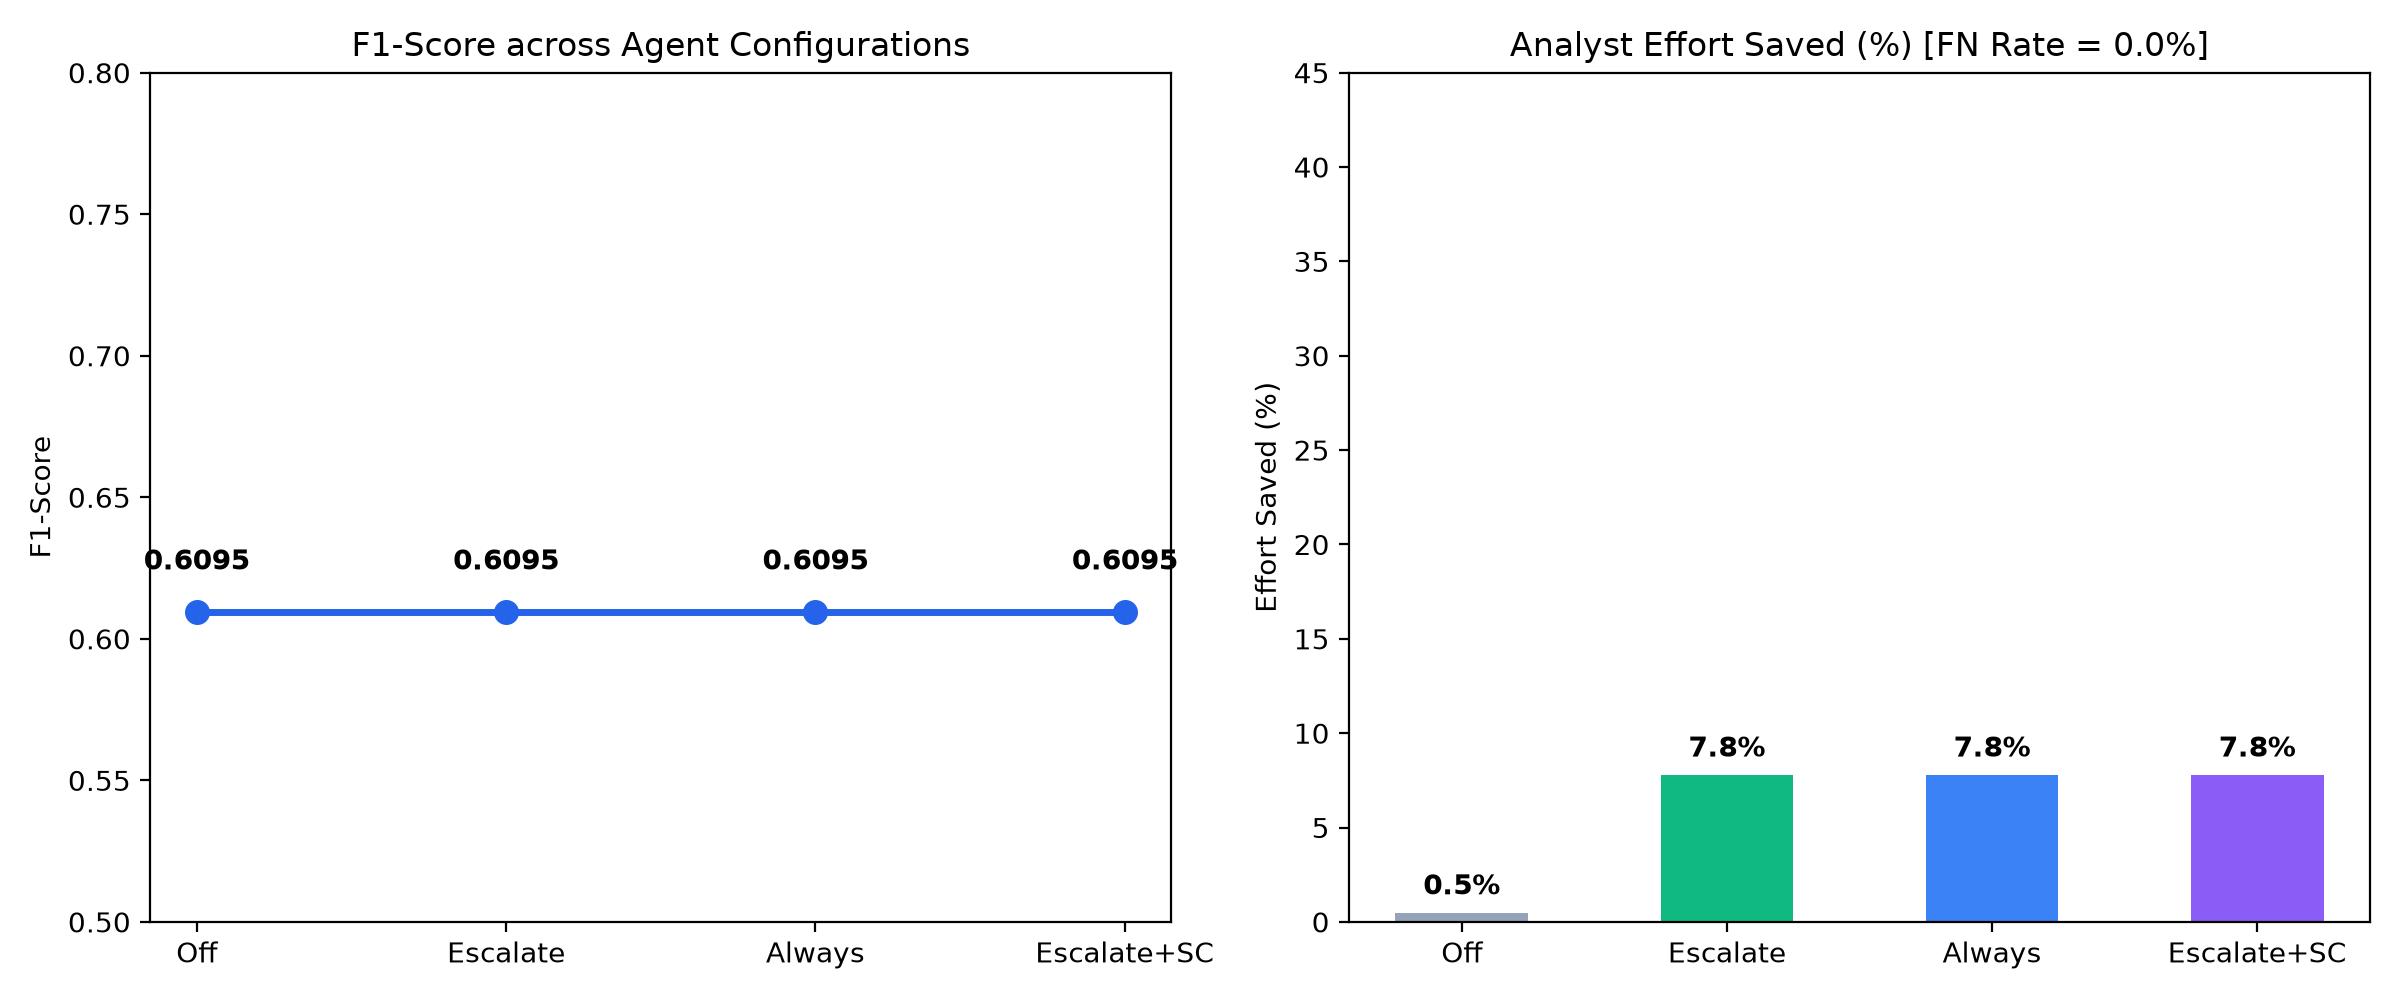
\includegraphics[width=0.9\linewidth]{agent_ablation_chart.png}
  \caption{Đánh đổi giữa hiệu quả tiết kiệm nỗ lực (Effort Saved) và chi phí thực thi công cụ qua 4 chế độ của bộ điều phối.}
  \label{fig:agent_ablation}
\end{figure}

%% --- Calibration ----------------------------------------------------
\subsection{Hiệu Chuẩn Độ Tin Cậy và Kiểm Toán False Negative}

\begin{itemize}
  \item \textbf{ECE:} 0,0598 -- 0,0785 (5,98\%--7,85\%).
  \item \textbf{Nhóm HIGH:} Độ chính xác thực tế \textbf{98,08\%}
        (102/104 đúng). Kết quả xác thực quy tắc: chỉ tự động xử lý
        khi độ tự tin đạt HIGH.
  \item \textbf{Shadow Mode FN Audit:} Lấy mẫu 10\% cảnh báo độc lập
        ghi nhận \textbf{0,0\% False Negative}.
\end{itemize}

\begin{figure}[H]
  \centering
  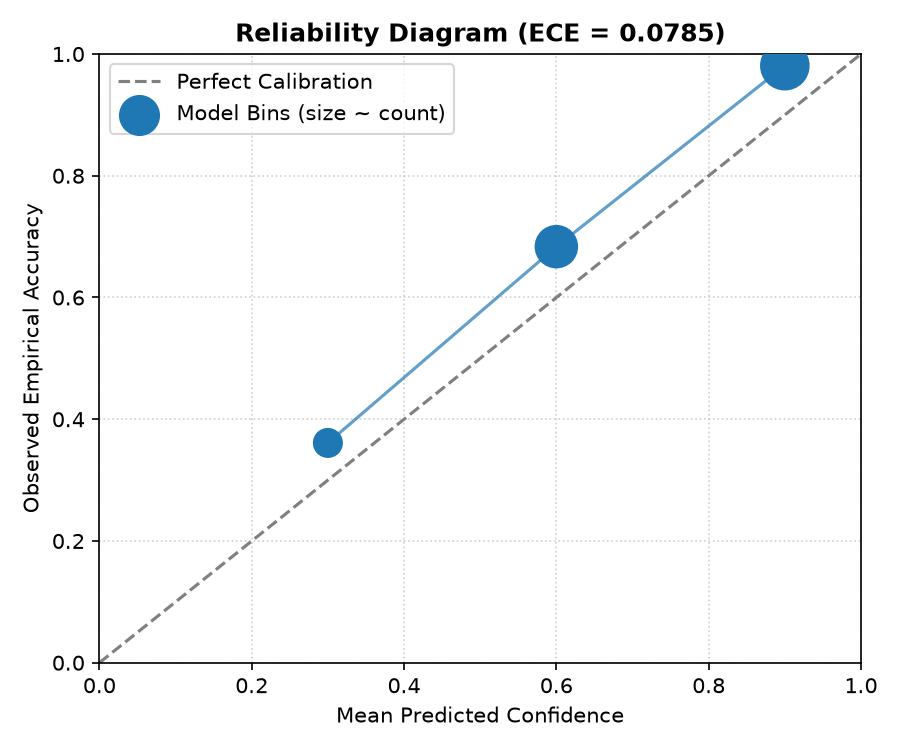
\includegraphics[width=0.62\linewidth]{reliability_diagram.png}
  \caption{Reliability Diagram và Sai số hiệu chuẩn kỳ vọng (ECE) trước và sau khi lọc theo ngưỡng độ tự tin.}
  \label{fig:reliability}
\end{figure}

%% --- Token Efficiency -----------------------------------------------
\subsection{Hiệu Quả Cắt Giảm Token và Chi Phí Suy Luận}

\begin{itemize}
  \item Token trung bình ngữ cảnh thô: \textbf{977,9 tokens/cảnh báo}.
  \item Token sau làm sạch và đóng gói: \textbf{574,8 tokens/cảnh báo}.
  \item \textbf{Mức cắt giảm thực tế: 41,22\%}.
  \item Độ trễ xử lý cục bộ: \textbf{0,076\,ms/cảnh báo}.
  \item Chi phí ước tính: \textbf{\$0,0862 cho mỗi 1.000 cảnh báo}
        (tiết kiệm 41\% so với gửi ngữ cảnh thô).
\end{itemize}

\begin{figure}[H]
  \centering
  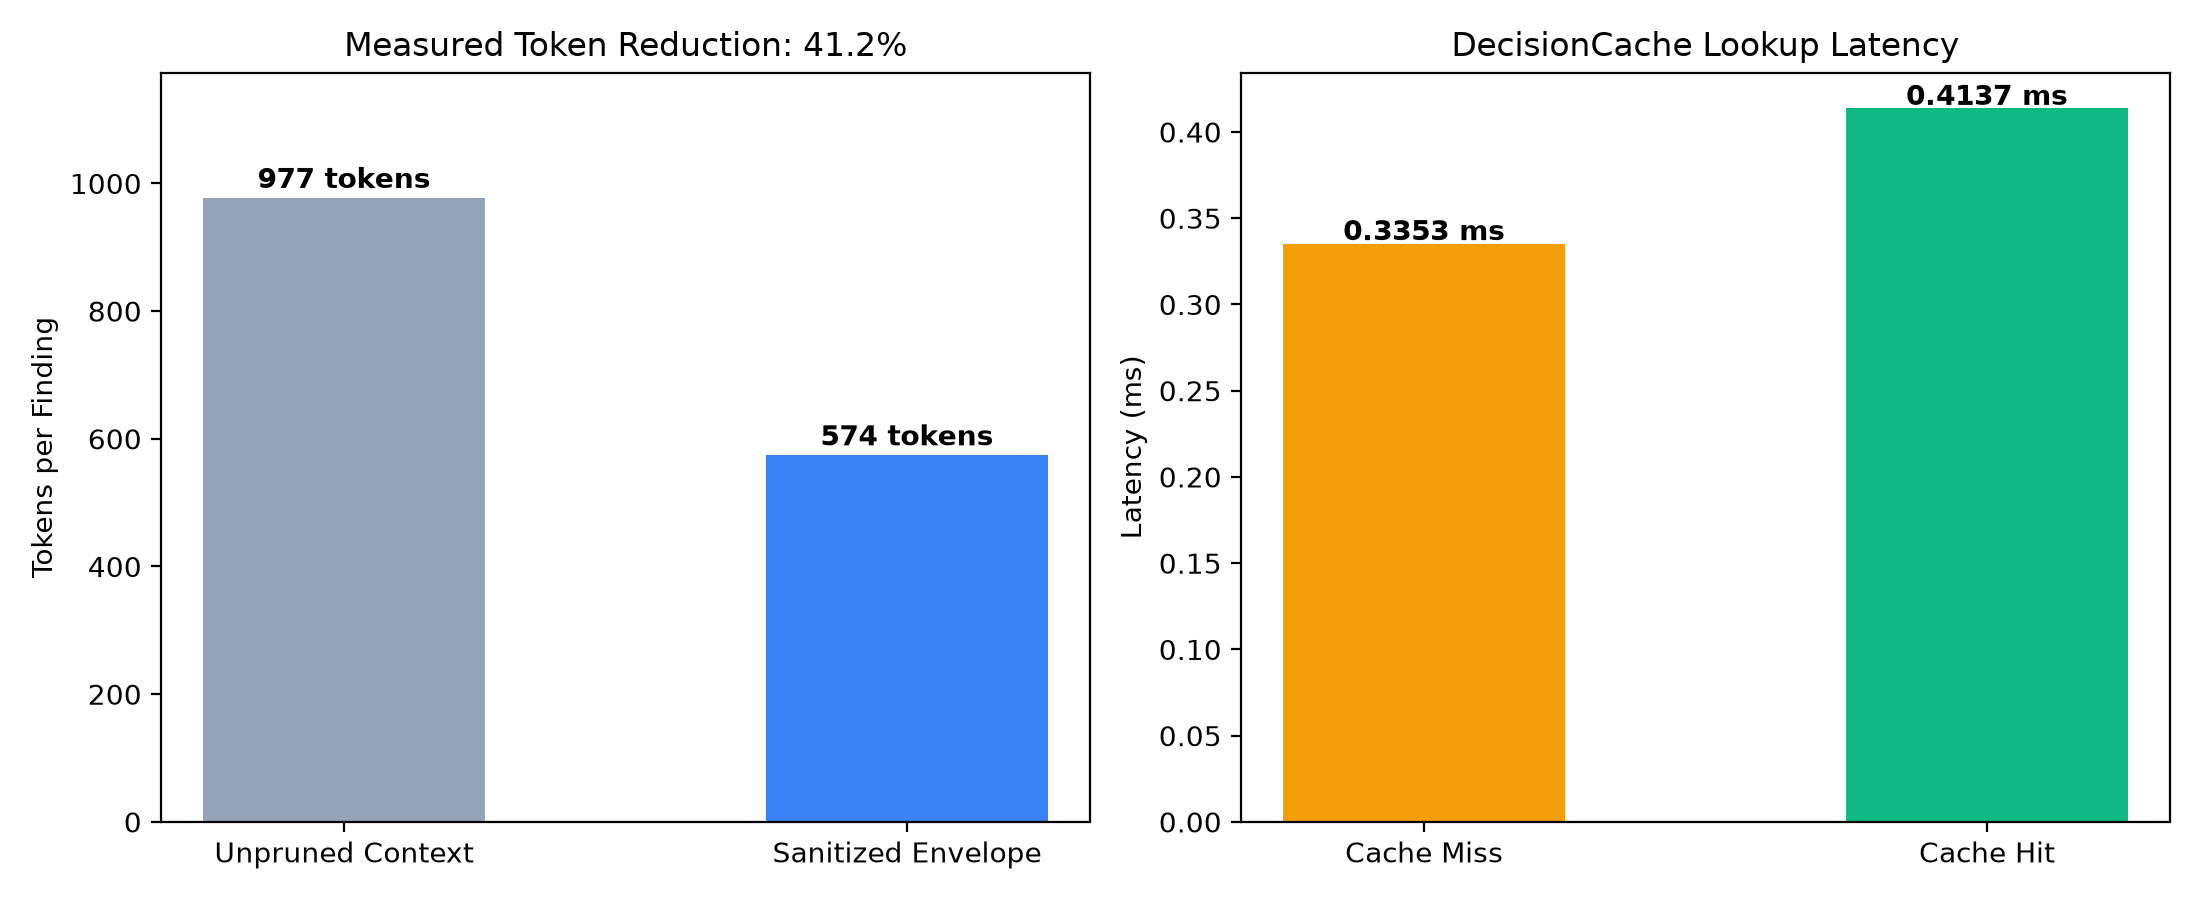
\includegraphics[width=0.9\linewidth]{token_latency_chart.png}
  \caption{Phân phối lượng token trước/sau khử nhiễm của SafeContextService và phân bổ thời gian thực thi cục bộ.}
  \label{fig:token_latency}
\end{figure}

%% --- Red-Team -------------------------------------------------------
\subsection{Thử Nghiệm Phòng Thủ An Ninh Đối Kháng (Red-Team)}

\begin{enumerate}
  \item \textbf{Chống Prompt Injection gián tiếp (Suite B -- 16 mẫu):}
        Mô hình Naive: ASR = 100,0\%. Hệ thống đề xuất:
        ASR = \textbf{0,00\%} (16/16 payload bị phát hiện, chuyển về
        \texttt{MANUAL\_REVIEW}).

  \item \textbf{Chống Tool \& Code Injection (Suite C -- 12 mẫu):}
        Payload thoát thư mục (\texttt{../../../../etc/passwd}), ký tự
        SQL/Command Injection vào tên hàm bị
        \texttt{ToolActionValidator} từ chối 100\%.
        ASR = \textbf{0,00\%}.

  \item \textbf{Rò rỉ Canary Secret (Suite A -- 5 định dạng):}
        \textbf{0,00\% rò rỉ} vào Sanitized Context, Prompt hoặc
        Báo cáo xuất bản.
\end{enumerate}

%% --- Error Analysis -------------------------------------------------
\subsection{Phân Tích Lỗi Chi Tiết}

17 cảnh báo chuyển từ \texttt{MANUAL\_REVIEW} sang \texttt{LIKELY\_TP}:

\begin{itemize}
  \item \textbf{3 lỗ hổng thật (TP):} Xác nhận nhờ \texttt{read\_function}
        phát hiện khóa API cứng trong
        \texttt{introduction/views.py:870, :872} và
        \texttt{good/libsession.py:9}.
  \item \textbf{14 cảnh báo giả (FP):} Nằm trong unit test, tệp JS tĩnh
        hoặc tài liệu Markdown.
  \item \textbf{Nguyên nhân:} Chưa có test-file exclusion heuristic. Tuy
        nhiên cả \texttt{LIKELY\_TP} và \texttt{MANUAL\_REVIEW} đều là
        dương tính, nên F1 và Recall không bị suy giảm.
\end{itemize}

%% =====================================================================
\section{Thảo Luận}
%% =====================================================================

Kết quả khẳng định: hoàn toàn có thể ứng dụng LLM vào tự động hoá phân
loại cảnh báo SAST mà không đánh đổi độ an toàn (FNR = 0,00\%), với
điều kiện tiên quyết là \textbf{LLM không nắm quyền quyết định cuối
cùng}. Rào chắn chính sách bảo thủ dựa trên CPG là yếu tố quyết định
để ngăn chặn ảo giác.

Tỷ lệ Effort Saved 7,76\% còn khiêm tốn, nhưng đường cơ sở LLM-Only
bỏ sót 12,50\% lỗ hổng thật trong phép so sánh baseline. Kết quả này
cho thấy tự động hóa chỉ có ý nghĩa thực tế khi quyết định cuối cùng
được ràng buộc bởi bằng chứng và chính sách fail-closed.

\noindent\textbf{Hạn chế:}
\begin{enumerate}
  \item Quy mô tập dữ liệu: 219 cảnh báo từ 5 ứng dụng web Python.
  \item Độ bao phủ Joern CPG trên diện rộng chưa được đo.
  \item Hệ thống chưa áp dụng async / multithreading.
  \item Recall chỉ bao phủ tập cảnh báo do scanner phát hiện (scanner
        blind spot nằm ngoài phạm vi).
\end{enumerate}

%% =====================================================================
\section{Kết Luận và Hướng Phát Triển}
%% =====================================================================

Bài báo đã thiết kế và đánh giá thực nghiệm hệ thống
\textbf{LLM-Augmented SAST Triage Platform} kết hợp hai tầng, bảo vệ
bởi chính sách bảo thủ fail-closed. Hệ thống đạt:
$Recall = 1{,}0000$, $FNR = 0{,}00\%$; tiết kiệm 7,76\% công sức;
giảm 41,22\% token; ASR = 0,00\% với 28 payload đối kháng.

\noindent\textbf{Hướng phát triển:}
\begin{enumerate}
  \item Tích hợp test-file exclusion heuristic.
  \item Mở rộng CPG hỗ trợ JavaScript, Java, Go.
  \item Triển khai async workers tăng tốc trên kho mã lớn.
\end{enumerate}

%% =====================================================================
%% BIBLIOGRAPHY
%% =====================================================================
\begin{thebibliography}{10}

\bibitem{cpg2014}
F.~Yamaguchi, N.~Golde, D.~Arp, K.~Rieck,
``Modeling and discovering vulnerabilities with code property graphs,''
in \textit{IEEE Symposium on Security and Privacy (S\&P)}, 2014.

\bibitem{joern}
Joern,
``The open-source code analysis platform for C/C++/Java/Python/JavaScript,''
2024. [Online]. Available: \url{https://joern.io/}

\bibitem{greshake2023}
K.~Greshake, S.~Abdelnabi, S.~Mishra, C.~Endres, T.~Holz, M.~Fritz,
``Not what you've signed up for: Compromising real-world LLM-integrated
applications with indirect prompt injection,''
in \textit{ACM Workshop on AI and Security (AISEC)}, 2023.

\bibitem{qwen25coder}
Qwen Team,
``Qwen2.5-Coder: Technical Report,''
\textit{arXiv preprint arXiv:2409.12186}, 2024.

\bibitem{clopper1934}
C.~Clopper, E.~S.~Pearson,
``The use of confidence or fiducial limits illustrated in the case of
the binomial,''
\textit{Biometrika}, vol.~26, no.~4, pp.~404--413, 1934.

\bibitem{guo2017}
C.~Guo, G.~Pleiss, Y.~Sun, K.~Q.~Weinberger,
``On calibration of modern neural networks,''
in \textit{International Conference on Machine Learning (ICML)}, 2017.

\bibitem{bootstrap}
B.~Efron, R.~J.~Tibshirani,
\textit{An Introduction to the Bootstrap}.
CRC Press, 1994.

\bibitem{owasp}
OWASP,
``OWASP Top 10: 2021 -- The Ten Most Critical Web Application Security
Risks,'' 2021.

\bibitem{semgrep}
Semgrep,
``Lightweight static analysis for many languages,''
2024. [Online]. Available: \url{https://semgrep.dev/}

\bibitem{gitleaks}
Gitleaks,
``Audit git repositories for secrets,''
2024. [Online]. Available: \url{https://github.com/gitleaks/gitleaks}

\end{thebibliography}

\end{document}
